%%%%%%%%%%%%%%%%%%%%%%%%%%%%%%%%%%%%%%%%%%%%%%%%%%%%%%%%%%%%%%%%%%%%%%%%%%%%%%%%
%2345678901234567890123456789012345678901234567890123456789012345678901234567890
%        1         2         3         4         5         6         7         8
%% memo.tex
%% V1.1
%% 2017/10/203
%% by Prof. Rui Santos Cruz
%% based on a template created by Rob Oakes
%%%%%%%%%%%%%%%%%%%%%%%%%%%%%%%%%%%%%%%%%%%%%%%%%%%%%%%%%%%%%%%%%%%%%%%%%%%%%%%%
\documentclass[a4paper,12pt]{texMemo}
% --> Please Choose the MAIN LANGUAGE for the document in package BABEL
% --> by replacing "main=" in language name selector. Default is "main=english"
\usepackage{graphicx}
\usepackage{float}
\usepackage{hyperref}
\usepackage[english,main=portuguese]{babel} % Defines Main language
\usepackage[utf8]{inputenc}
\usepackage{iflang}
\usepackage{ifthen}
\usepackage{parskip}
\setlength{\parindent}{15pt}
\logo{
\includegraphics[width=0.3\textwidth]{logo.png}} % Logo
%%%%%%%%%%%%%%%%%%%%%%%%%%%%%%%%%%%%%%%%%%%%%%%%%%%%%%%%%%%%%%%%%%%%%%%%%%%%%%%%
%	MEMO INFORMATION --> Write your info in the following tags.
%%%%%%%%%%%%%%%%%%%%%%%%%%%%%%%%%%%%%%%%%%%%%%%%%%%%%%%%%%%%%%%%%%%%%%%%%%%%%%%%
\memofrom{All ZJUI/ZJE Associate Sophomore (2020)} % Sender(s) Name
\memoid{Jack BAI, \textsc{Hepta Workshop}} % Student ID
\memocourse{Haob.19@intl.zju.edu.cn / WeChat \textit{Jackgetup}} % Course Name, or abbreviated acronym
\memosubject{User Interface Designer, Front-end Engineer, FB Interaction Engineer, Operation Engineer, Bursar Correspondent, Penetration Testing Engineer(or \textit{Kali} Hacker), Product Manager} % Subject
\memodate{\today} % Date, -> set to \today for automatically print todays date
%%%%%%%%%%%%%%%%%%%%%%%%%%%%%%%%%%%%%%%%%%%%%%%%%%%%%%%%%%%%%%%%%%%%%%%%%%%%%%%%
\maketitle % Print the memo header information
%%%%%%%%%%%%%%%%%%%%%%%%%%%%%%%%%%%%%%%%%%%%%%%%%%%%%%%%%%%%%%%%%%%%%%%%%%%%%%%%
%	MEMO CONTENT --> Your content is written here
%%%%%%%%%%%%%%%%%%%%%%%%%%%%%%%%%%%%%%%%%%%%%%%%%%%%%%%%%%%%%%%%%%%%%%%%%%%%%%%%
\begin{document}
Hi sophomore students, it's my honor to give you the recruitment letter to join the BB-CWL Project by \textsc{Hepta Workshop}. This project is associated with the \textsc{Information \& Technology Service}, which focuses on the transplant of some of BlackBoards's functionalities onto WeChat Applets. This recruitment letter also looks for candidate launchpad copartners for \textsc{Hepta Workshop}. Shown below are the positions and corresponding skills you need to command.


\begin{enumerate}



\item User Interface Designer (1 person): this is an \textbf{urgent} position, which means you're likely to be quickly accepted if you have corresponding skills. This position needs a relatively high level of aesthetical perception and design inspiration. If you join this position, you're going to design the user interface on our WeChat Applets. For example, you need to select from A and B, and tell why you think it's more aesthetically attracting. \\


\begin{figure}[H]
  \begin{minipage}[t]{0.5\linewidth}
    \centering
    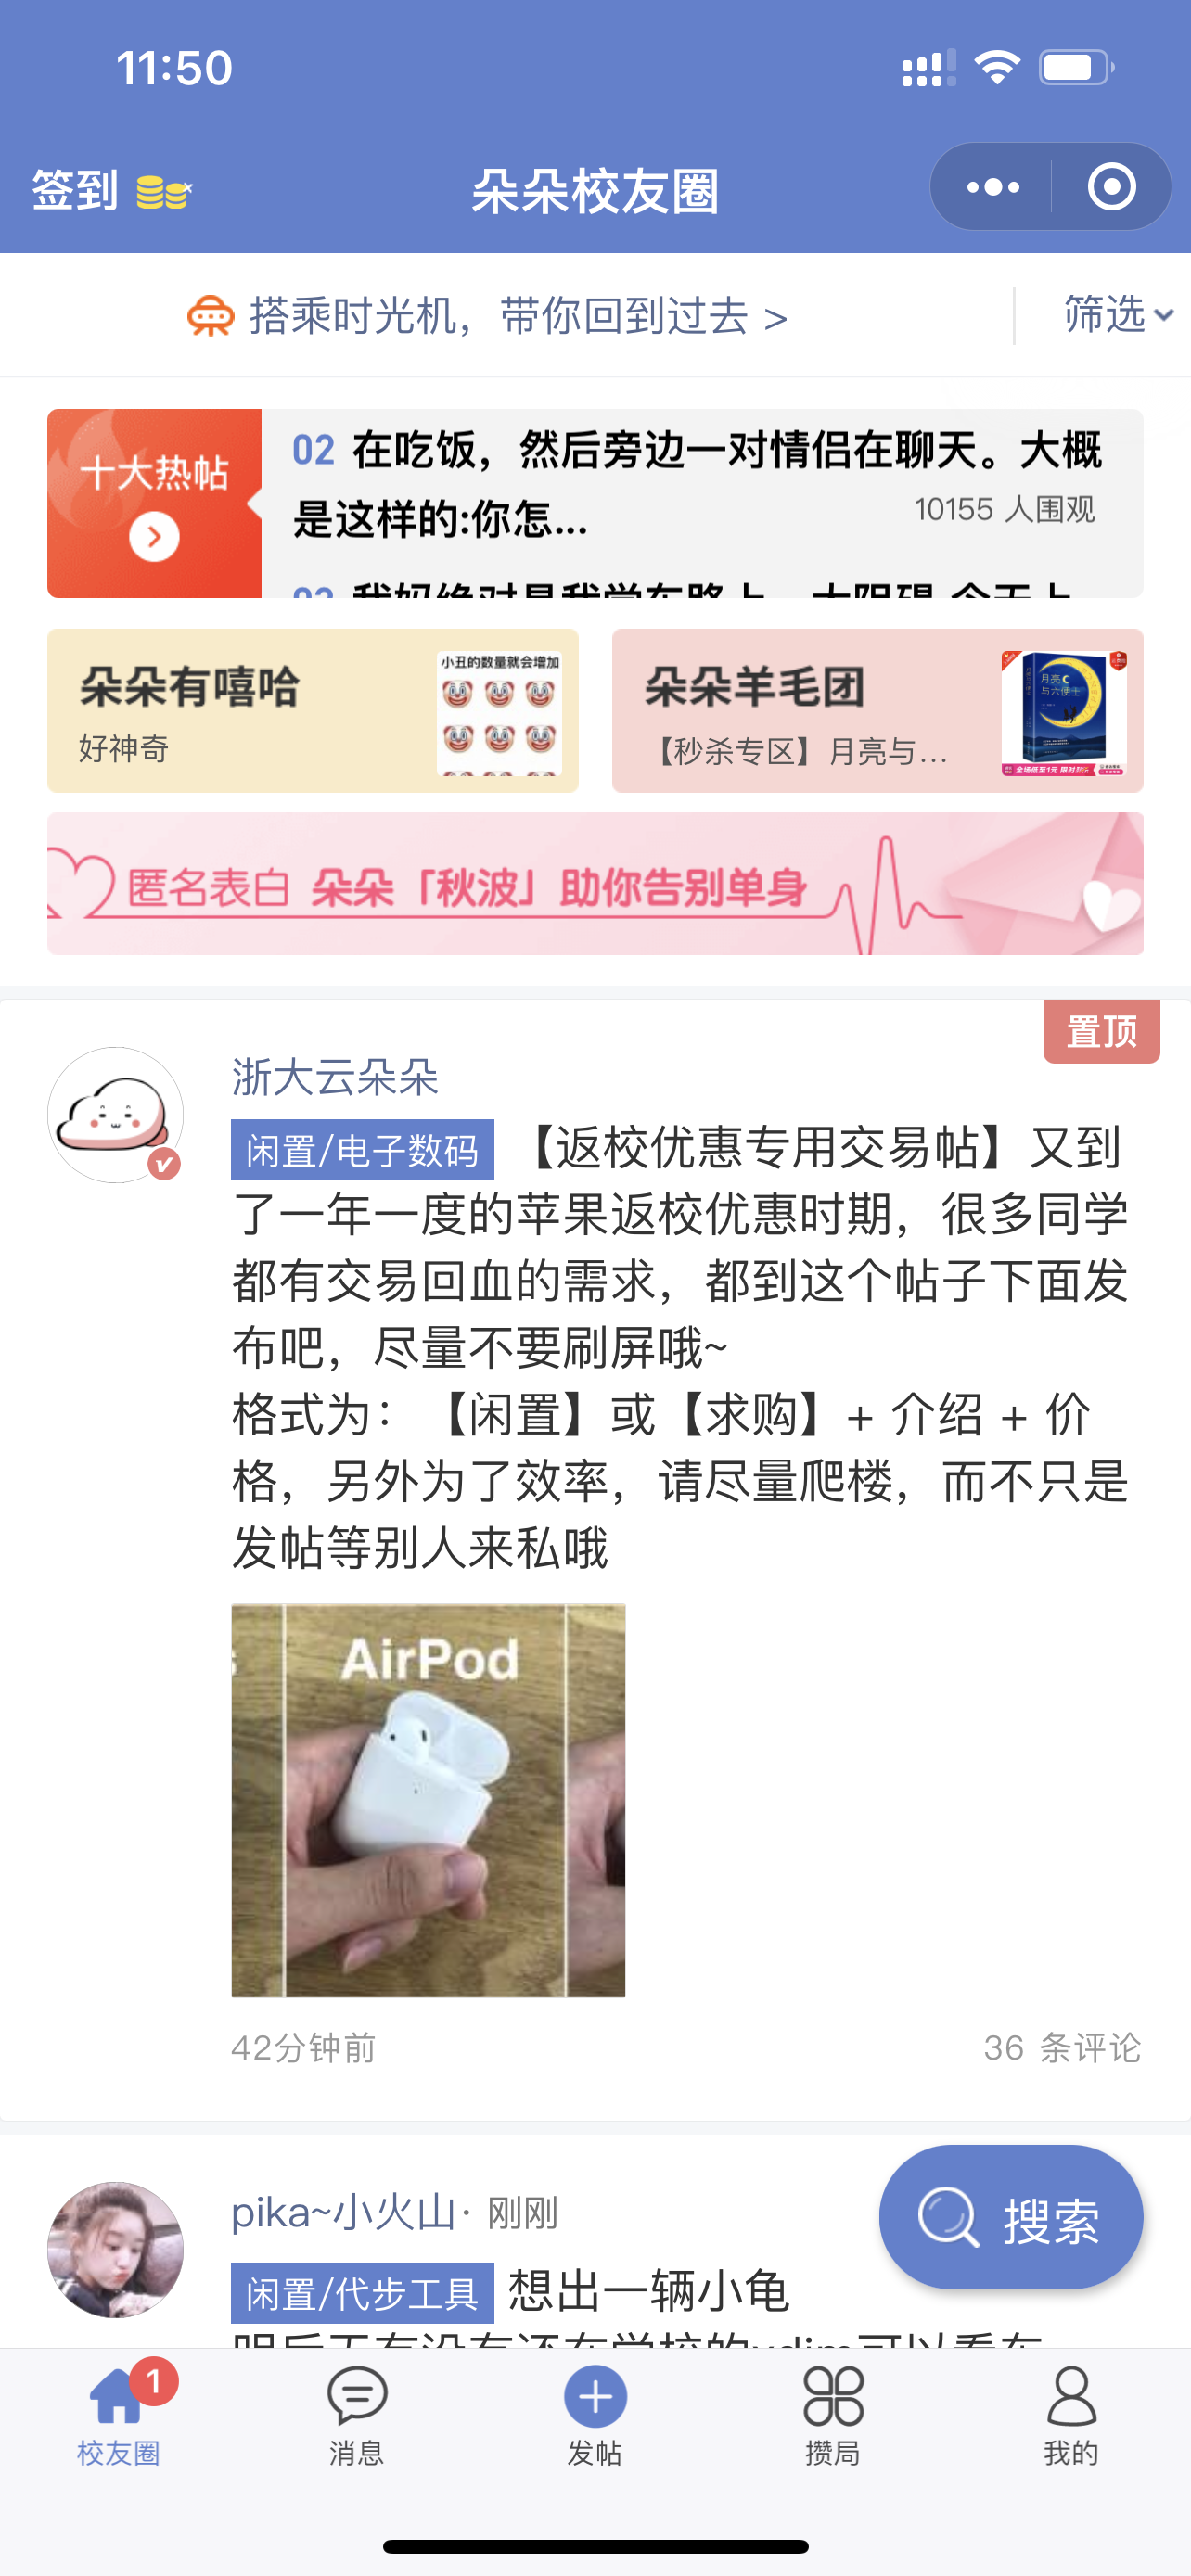
\includegraphics[scale=0.07]{IMG_2920.PNG}
    \caption{Yun Duoduo WA}
    \label{fig:side:a}
  \end{minipage}%
  \begin{minipage}[t]{0.5\linewidth}
    \centering
    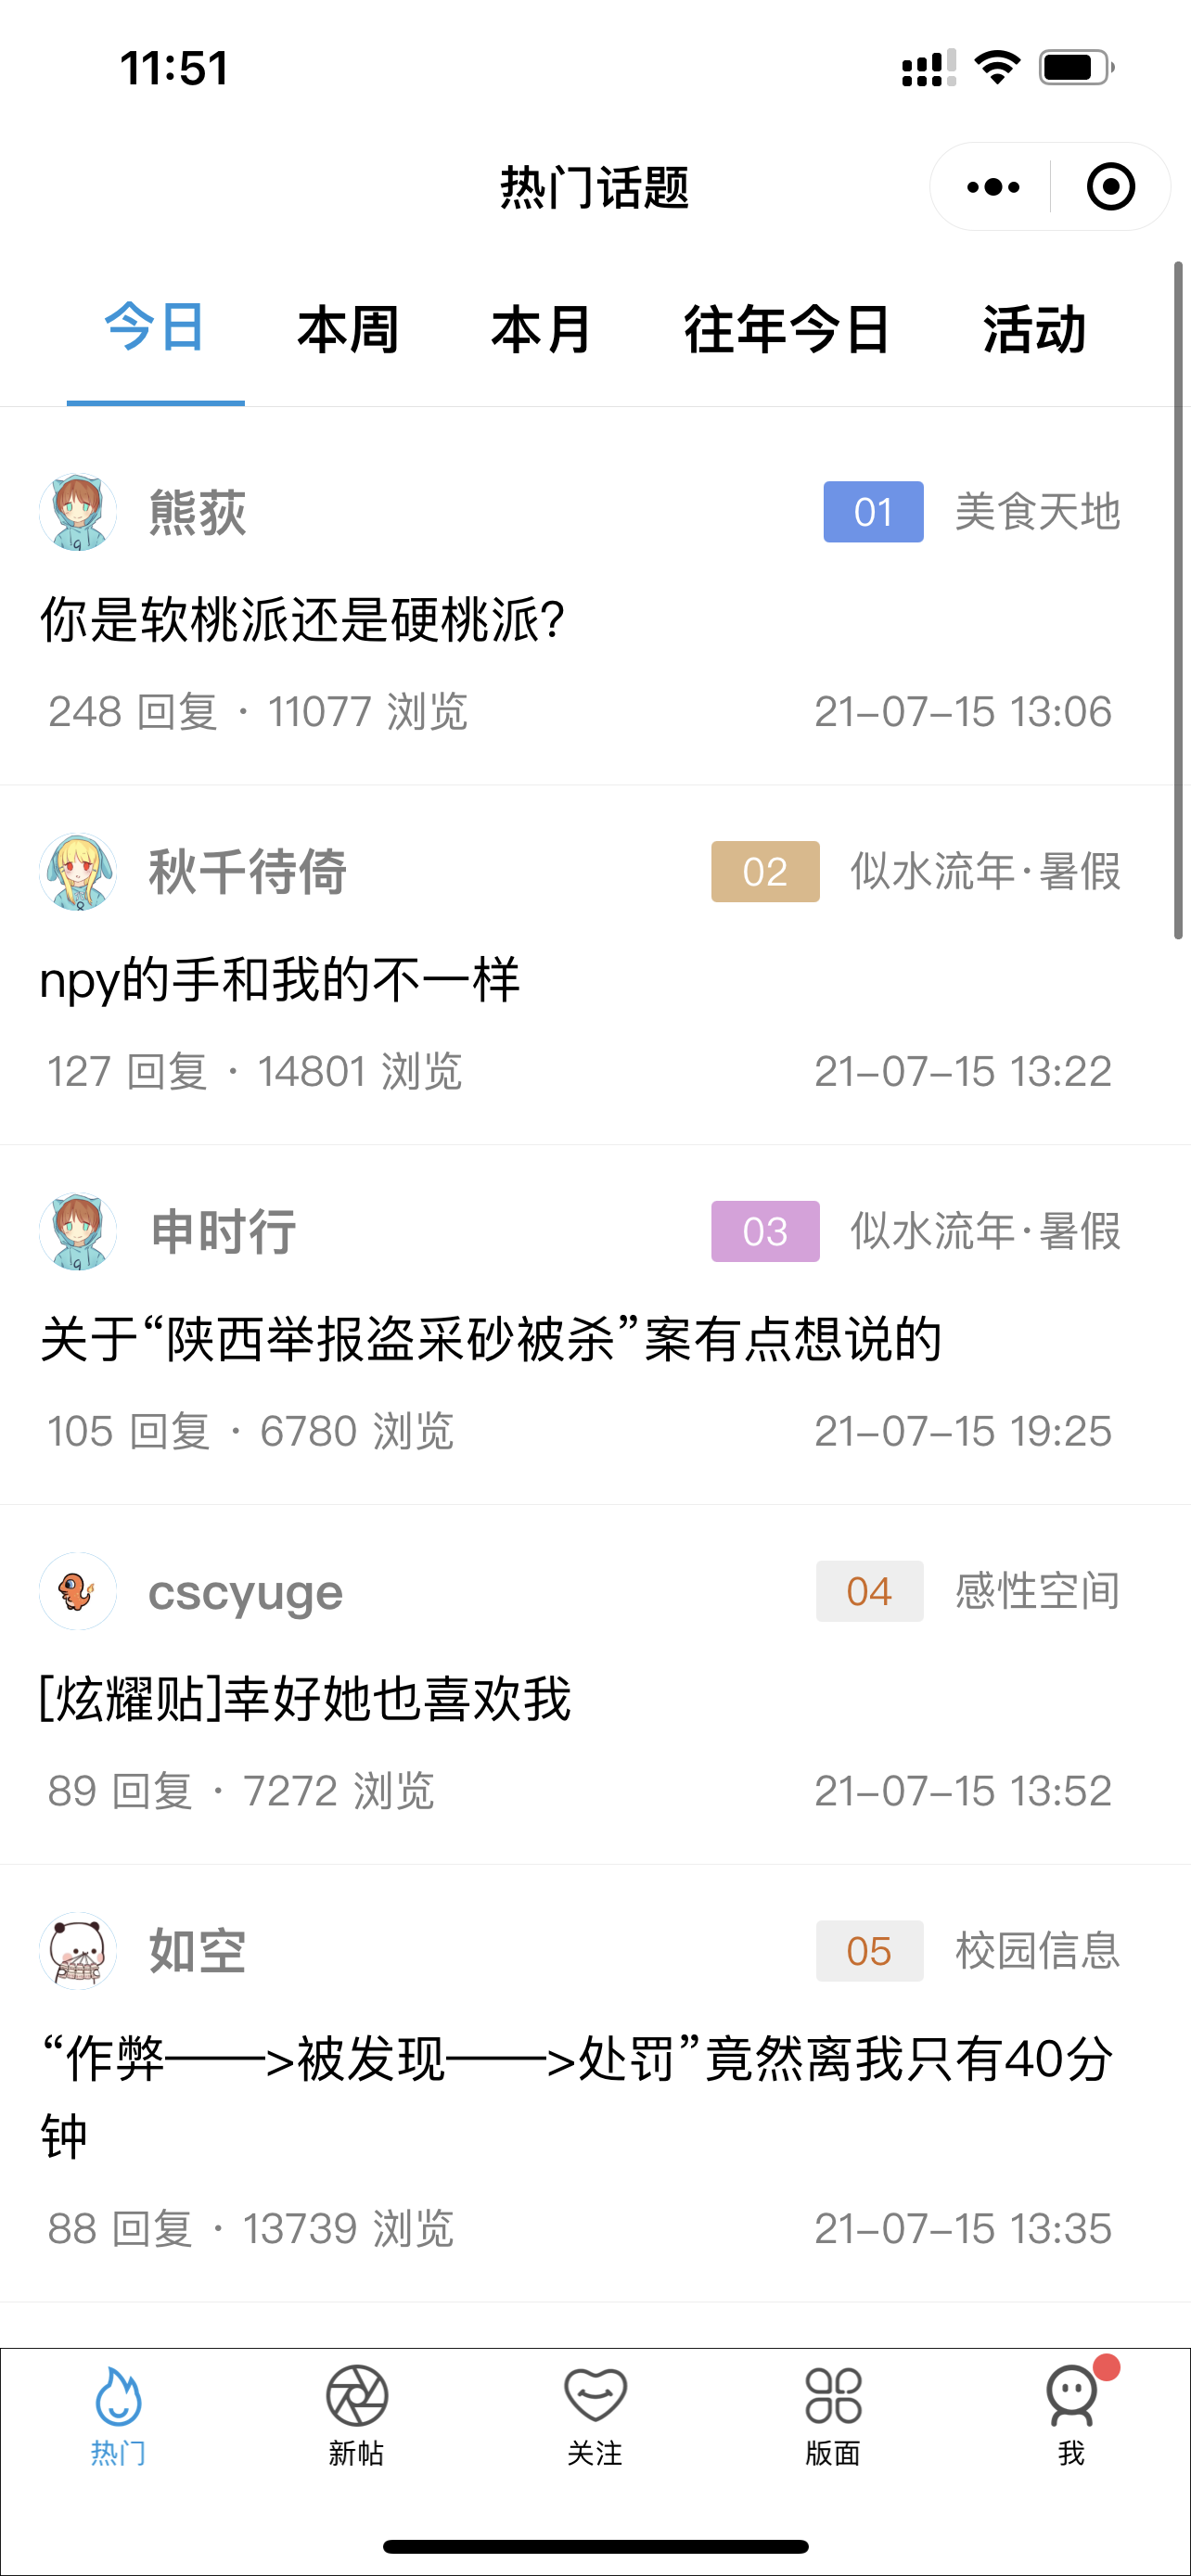
\includegraphics[scale=0.07]{IMG_2921.PNG}
    \caption{CC98 WA}
    \label{fig:side:b}
  \end{minipage}
\end{figure}


\newpage



\item Bursar/Correspondent (1 person): this is an \textbf{urgent} position, which means you're likely to be quickly accepted if you have corresponding skills. This position requires you to obey certain patience to communicate with other organizations and counting bursar in Hepta Workshop. Girls are preferred for this position. If you're passionate about writing passages and propagandizing, we're happy to accept you,
\item \textbf{Product Manager} (1 person): this is an \textbf{demanding} position, which means you need to have a relative high level of agility of processing projects and arranging group tasks. Students in the Student Union and Residential Union are preferred, and every student coming for this position will be strictly examined for their ability.
\item Front-end Engineer (1 person): this is a back-up position, which means that you do not need to master an industrial level of technique, and can be listed as a developing target. If you join you're going to learn about \textsc{Vue.js, Html5, Css3} until you bear the ability for industrial production.
\item Front-Back-end Interaction Engineer (1 person): this is a back-up position, which means that you do not need to master an industrial level of technique, and can be listed as a developing target. If you join you're going to learn about \textsc{Node.js, JavaScript, MySQL} until you bear the ability for industrial production.
\item Operation Engineer (1 person): this is a back-up position, which means that you do not need to master an industrial level of technique, and can be listed as a developing target. If you join you're going to learn about \textsc{CentOS Linux, Server Operations, Computer Network} until you bear the ability for industrial production.
\item Penetration Testing Engineer / \textit{Kali} Hacker(1 person): this is a back-up position, which means that you do not need to master an industrial level of technique, and can be listed as a developing target. If you join you're going to learn about \textsc{Kali Hacking Tech, Web Penetration, Network Attack/Defense} until you bear the ability for industrial production.

\end{enumerate}

If you have willingness to admit to any of the above, please E-mail me or contact me through WeChat \textit{Jackgetup} with your in-progress/done projects and your skills hitherto. Our Human Resource Department is likely to hold an interview with all applicants and figure out candidates.

%%%%%%%%%%%%%%%%%%%%%%%%%%%%%%%%%%%%%%%%%%%%%%%%%%%%%%%%%%%%%%%%%%%%%%%%%%%%%%%%
\end{document}